\documentclass[11pt,preprint, authoryear]{elsarticle}

\usepackage{lmodern}
%%%% My spacing
\usepackage{setspace}
\setstretch{1.2}
\DeclareMathSizes{12}{14}{10}{10}

% Wrap around which gives all figures included the [H] command, or places it "here". This can be tedious to code in Rmarkdown.
\usepackage{float}
\let\origfigure\figure
\let\endorigfigure\endfigure
\renewenvironment{figure}[1][2] {
    \expandafter\origfigure\expandafter[H]
} {
    \endorigfigure
}

\let\origtable\table
\let\endorigtable\endtable
\renewenvironment{table}[1][2] {
    \expandafter\origtable\expandafter[H]
} {
    \endorigtable
}


\usepackage{ifxetex,ifluatex}
\usepackage{fixltx2e} % provides \textsubscript
\ifnum 0\ifxetex 1\fi\ifluatex 1\fi=0 % if pdftex
  \usepackage[T1]{fontenc}
  \usepackage[utf8]{inputenc}
\else % if luatex or xelatex
  \ifxetex
    \usepackage{mathspec}
    \usepackage{xltxtra,xunicode}
  \else
    \usepackage{fontspec}
  \fi
  \defaultfontfeatures{Mapping=tex-text,Scale=MatchLowercase}
  \newcommand{\euro}{€}
\fi

\usepackage{amssymb, amsmath, amsthm, amsfonts}

\def\bibsection{\section*{References}} %%% Make "References" appear before bibliography


\usepackage[round]{natbib}

\usepackage{longtable}
\usepackage[margin=2.3cm,bottom=2cm,top=2.5cm, includefoot]{geometry}
\usepackage{fancyhdr}
\usepackage[bottom, hang, flushmargin]{footmisc}
\usepackage{graphicx}
\numberwithin{equation}{section}
\numberwithin{figure}{section}
\numberwithin{table}{section}
\setlength{\parindent}{0cm}
\setlength{\parskip}{1.3ex plus 0.5ex minus 0.3ex}
\usepackage{textcomp}
\renewcommand{\headrulewidth}{0.2pt}
\renewcommand{\footrulewidth}{0.3pt}

\usepackage{array}
\newcolumntype{x}[1]{>{\centering\arraybackslash\hspace{0pt}}p{#1}}

%%%%  Remove the "preprint submitted to" part. Don't worry about this either, it just looks better without it:
\makeatletter
\def\ps@pprintTitle{%
  \let\@oddhead\@empty
  \let\@evenhead\@empty
  \let\@oddfoot\@empty
  \let\@evenfoot\@oddfoot
}
\makeatother

 \def\tightlist{} % This allows for subbullets!

\usepackage{hyperref}
\hypersetup{breaklinks=true,
            bookmarks=true,
            colorlinks=true,
            citecolor=blue,
            urlcolor=blue,
            linkcolor=blue,
            pdfborder={0 0 0}}


% The following packages allow huxtable to work:
\usepackage{siunitx}
\usepackage{multirow}
\usepackage{hhline}
\usepackage{calc}
\usepackage{tabularx}
\usepackage{booktabs}
\usepackage{caption}


\newenvironment{columns}[1][]{}{}

\newenvironment{column}[1]{\begin{minipage}{#1}\ignorespaces}{%
\end{minipage}
\ifhmode\unskip\fi
\aftergroup\useignorespacesandallpars}

\def\useignorespacesandallpars#1\ignorespaces\fi{%
#1\fi\ignorespacesandallpars}

\makeatletter
\def\ignorespacesandallpars{%
  \@ifnextchar\par
    {\expandafter\ignorespacesandallpars\@gobble}%
    {}%
}
\makeatother

\newenvironment{CSLReferences}[2]{%
}

\urlstyle{same}  % don't use monospace font for urls
\setlength{\parindent}{0pt}
\setlength{\parskip}{6pt plus 2pt minus 1pt}
\setlength{\emergencystretch}{3em}  % prevent overfull lines
\setcounter{secnumdepth}{5}

%%% Use protect on footnotes to avoid problems with footnotes in titles
\let\rmarkdownfootnote\footnote%
\def\footnote{\protect\rmarkdownfootnote}
\IfFileExists{upquote.sty}{\usepackage{upquote}}{}

%%% Include extra packages specified by user

%%% Hard setting column skips for reports - this ensures greater consistency and control over the length settings in the document.
%% page layout
%% paragraphs
\setlength{\baselineskip}{12pt plus 0pt minus 0pt}
\setlength{\parskip}{12pt plus 0pt minus 0pt}
\setlength{\parindent}{0pt plus 0pt minus 0pt}
%% floats
\setlength{\floatsep}{12pt plus 0 pt minus 0pt}
\setlength{\textfloatsep}{20pt plus 0pt minus 0pt}
\setlength{\intextsep}{14pt plus 0pt minus 0pt}
\setlength{\dbltextfloatsep}{20pt plus 0pt minus 0pt}
\setlength{\dblfloatsep}{14pt plus 0pt minus 0pt}
%% maths
\setlength{\abovedisplayskip}{12pt plus 0pt minus 0pt}
\setlength{\belowdisplayskip}{12pt plus 0pt minus 0pt}
%% lists
\setlength{\topsep}{10pt plus 0pt minus 0pt}
\setlength{\partopsep}{3pt plus 0pt minus 0pt}
\setlength{\itemsep}{5pt plus 0pt minus 0pt}
\setlength{\labelsep}{8mm plus 0mm minus 0mm}
\setlength{\parsep}{\the\parskip}
\setlength{\listparindent}{\the\parindent}
%% verbatim
\setlength{\fboxsep}{5pt plus 0pt minus 0pt}



\begin{document}



\begin{frontmatter}  %

\title{Question 3: Cold play and Metallica}

% Set to FALSE if wanting to remove title (for submission)




\author[Add1]{Austin Byrne}
\ead{22582053@sun.ac.za}





\address[Add1]{Music fenatic, Stellenbosch, South Africa}

\cortext[cor]{Corresponding author: Austin Byrne}

\begin{abstract}
\small{
Coldplay and Metallica are two of the greatest bands to have graced the
stage in recent decades. This paper attempts a comparisson of the two
bands in order to identify how a band can thrive theoughout generations.
In this report it is found that the two bands take different approaches
to their music. With varying attributes. What this comparisson report
establishes, is that, it is not possible to compare bands and make an
assuption od what their success will look like. Two very different bands
can survive through generations.
}
\end{abstract}

\vspace{1cm}





\vspace{0.5cm}

\end{frontmatter}

\setcounter{footnote}{0}



%________________________
% Header and Footers
%%%%%%%%%%%%%%%%%%%%%%%%%%%%%%%%%
\pagestyle{fancy}
\chead{}
\rhead{}
\lfoot{}
\rfoot{\footnotesize Page \thepage}
\lhead{}
%\rfoot{\footnotesize Page \thepage } % "e.g. Page 2"
\cfoot{}

%\setlength\headheight{30pt}
%%%%%%%%%%%%%%%%%%%%%%%%%%%%%%%%%
%________________________

\headsep 35pt % So that header does not go over title




\hypertarget{introduction}{%
\section{\texorpdfstring{Introduction
\label{Introduction}}{Introduction }}\label{introduction}}

This comparison report will take a deep dive into the various attributes
of Coldplay and Mettallica, such as, tempo, loudness and valence. this
comparison report attempts to understand if their are certain attributes
that ensure a bands success. Throughout this report it is found that the
two bands are very different and that there are no certainties when it
comes to what attributes a band needs to become successful.

\hypertarget{data}{%
\section{Data}\label{data}}

The data used is obtained from Spotify for the two bands of Coldplay and
Mettallica.

\hypertarget{graphical-representation-of-the-data}{%
\section{Graphical representation of the
data}\label{graphical-representation-of-the-data}}

\hypertarget{histogram-plotting-histograms-to-compare-the-distribution-of-tempo-values-for-coldplay-and-metallica-songs.}{%
\subsection{Histogram: Plotting histograms to Compare the distribution
of tempo values for Coldplay and Metallica
songs.}\label{histogram-plotting-histograms-to-compare-the-distribution-of-tempo-values-for-coldplay-and-metallica-songs.}}

\begin{figure}[H]

{\centering 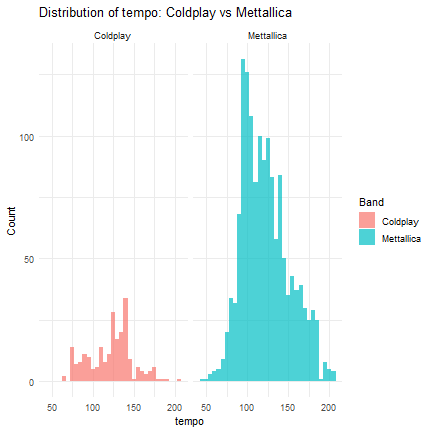
\includegraphics{Question-3_files/figure-latex/Figure 1-1} 

}

\caption{Tempo distribution \label{Figure1}}\label{fig:Figure 1}
\end{figure}

As can be seen in the above figure \ref{Figure1}, Mettallica has on
average a higher tempo count then that of Coldplay. What this means is
that Mettallica tends to play songs that are of a faster pace than
Coldplay. What can be taken from this output is that having a fast or
slow tempo on average for a band will not hint towards the band not
performing well over generations. This is because \ref{Figure1}, is
evidence towards two successful bands with differing tempos.

\hypertarget{violin-plot-compare-the-distribution-of-loudness-values-for-coldplay-and-metallica-songs-using-a-violin-plot.}{%
\subsection{Violin Plot: Compare the distribution of loudness values for
Coldplay and Metallica songs using a violin
plot.}\label{violin-plot-compare-the-distribution-of-loudness-values-for-coldplay-and-metallica-songs-using-a-violin-plot.}}

\begin{figure}[H]

{\centering 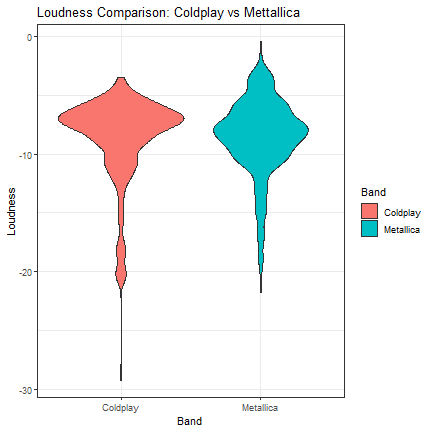
\includegraphics{Question-3_files/figure-latex/Figure 2-1} 

}

\caption{Loudness distribution \label{Figure2}}\label{fig:Figure 2}
\end{figure}

The purpose of the violin plot is too see the distribution of values. In
the case of \ref{Figure2}, we are analyzing the distribution of the
loudness variable for both Coldplay and Mettallica so as to compare how
loud the two bands on average play their music. As can be seen from
\ref{Figure2}, The mean values for both bands seem to be similar
however, the differences come in when we look at the tails. When
evaluating the tails of the \ref{Figure2} it is evident that Coldplay
tends to the lower volume while Mettallic on the occasion will play the
louder music.

\hypertarget{box-plot-compare-the-distribution-of-multiple-attributes-e.g.-danceability-energy-valence-between-coldplay-and-metallica-songs-using-box-plots-side-by-side.}{%
\subsection{Box Plot: Compare the distribution of multiple attributes
(e.g., danceability, energy, valence) between Coldplay and Metallica
songs using box plots side by
side.}\label{box-plot-compare-the-distribution-of-multiple-attributes-e.g.-danceability-energy-valence-between-coldplay-and-metallica-songs-using-box-plots-side-by-side.}}

\begin{figure}[H]

{\centering 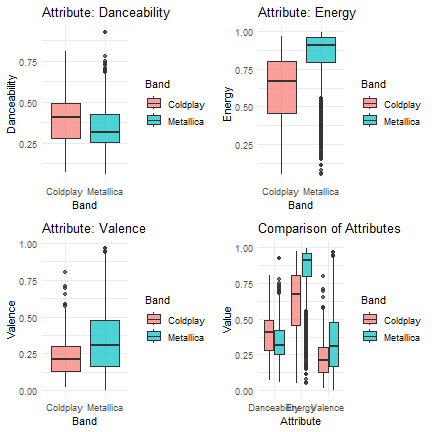
\includegraphics{Question-3_files/figure-latex/Figure 3-1} 

}

\caption{Attribute distribution \label{Figure3}}\label{fig:Figure 3}
\end{figure}

The final plot we will be looking at are some combined box plots which
aims to explain the differences in the attributes of danceability,
energy, and valence. As can be seen by \ref{Figure3}, Mettallica has a
lower danceability when compared to that of Coldplay, however, this is
the only measure where Mettallica lags Coldplay. On the other metrics
such as, energy and valence, Mettalic out performs Coldplay.

\hypertarget{conclusion}{%
\section{Conclusion}\label{conclusion}}

Therefore, to conclude, when comparring the two generational bands of
Coldplay and Mettallica it is evident that the bands are very different.
Mettalica tend to play louder music with more energy, while Coldplay
likes to play music that is softer but easier to dance too resulting in
the attraction of different crowds. Thus from the output seen, there is
no one formula that will lead to a band being successful. A band can be
successful being themselves and playing music they enjoy.

\bibliography{Tex/ref}





\end{document}
